\documentclass[border=1pt]{standalone}
\usepackage[T1]{fontenc}
\usepackage[scaled=0.92]{helvet}
\renewcommand{\familydefault}{\sfdefault}
\usepackage{amssymb}
\usepackage{tikz}
\usetikzlibrary{arrows.meta,calc,decorations.pathreplacing}
\renewcommand{\tiny}{\fontsize{6}{7}\selectfont}

% palette shared with the plots
\definecolor{navy}{HTML}{1F497D}
\definecolor{red}{HTML}{C0504D}
\definecolor{green}{HTML}{9BBB59}
\definecolor{cpuF}{HTML}{DCE6F2}
\definecolor{rtF}{HTML}{EBF1DE}
\definecolor{polF}{HTML}{D7E4BD}
\definecolor{mcF}{HTML}{E4DFEC}
\definecolor{dramF}{HTML}{F2F2F2}
\definecolor{fixF}{HTML}{D9D9D9}
\definecolor{t1}{HTML}{B9CDE5}
\definecolor{t2}{HTML}{D7E4BD}
\definecolor{t3}{HTML}{CCC1DA}
\definecolor{t4}{HTML}{FDE9D9}
\definecolor{t5}{HTML}{DAEEF3}
\definecolor{t6}{HTML}{FFF2CC}

\tikzset{
  box/.style={draw=black, line width=0.5pt, rectangle, anchor=north west},
  sub/.style={draw=black, line width=0.4pt, fill=white, rectangle, anchor=north west, align=center, font=\tiny, inner sep=1pt},
  num/.style={circle, fill=navy, text=white, font=\tiny\bfseries, inner sep=0.3pt, minimum size=7.5pt},
  arr/.style={-{Latex[length=3.5pt,width=3pt]}, line width=0.65pt},
  lbl/.style={font=\tiny, inner sep=1pt},
}

\begin{document}
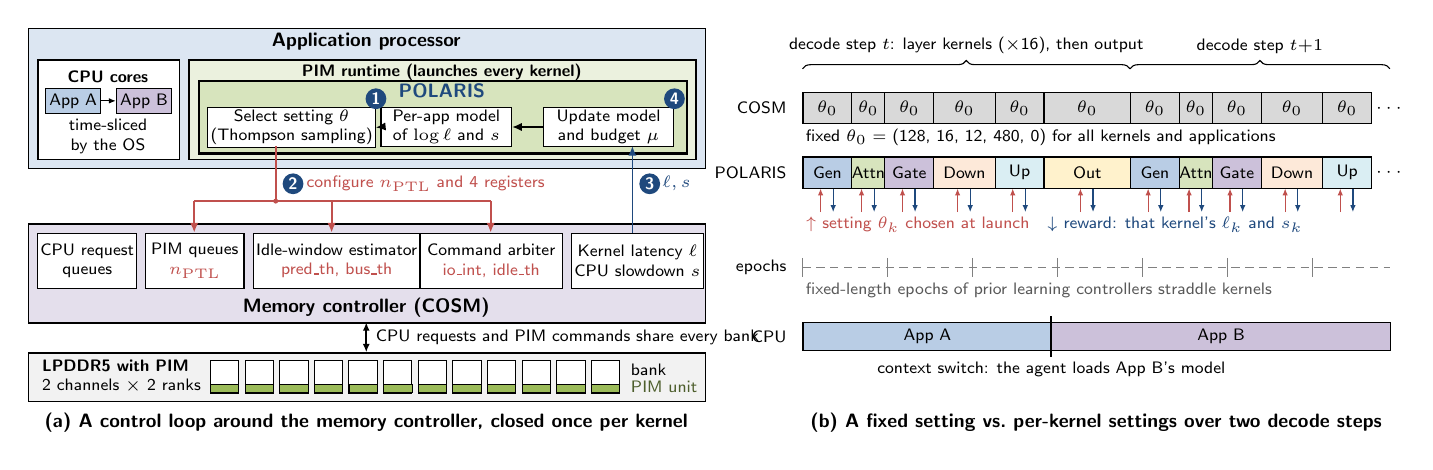
\begin{tikzpicture}[x=1cm, y=1cm]

%% =====================================================================
%% (a) POLARIS closes a loop around COSM's memory controller, once per PIM kernel
%% =====================================================================
% ---- application processor
\node[box, fill=cpuF, minimum width=8.6cm, minimum height=1.78cm] at (0,0) {};
\node[anchor=north, font=\scriptsize\bfseries, inner sep=1.5pt] at (4.30,0) {Application processor};

\node[box, fill=white, minimum width=1.80cm, minimum height=1.26cm] (cpu) at (0.12,-0.40) {};
\node[anchor=north, font=\tiny\bfseries] at (1.02,-0.42) {CPU cores};
\node[sub, fill=t1, minimum width=0.70cm, minimum height=0.32cm] (appa) at (0.22,-0.76) {App A};
\node[sub, fill=t3, minimum width=0.70cm, minimum height=0.32cm] (appb) at (1.12,-0.76) {App B};
\draw[-{Latex[length=2.5pt,width=2pt]}, line width=0.45pt] (appa.east) -- (appb.west);
\node[lbl, anchor=north, align=center] at (1.02,-1.12) {time-sliced\\by the OS};

\node[box, fill=rtF, minimum width=6.44cm, minimum height=1.26cm] (rt) at (2.04,-0.40) {};
\node[anchor=north, font=\tiny\bfseries, inner sep=1.5pt] at (5.26,-0.40) {PIM runtime (launches every kernel)};
\node[box, fill=polF, line width=0.9pt, minimum width=6.20cm, minimum height=0.92cm] (pol) at (2.16,-0.66) {};
\node[anchor=north, font=\scriptsize\bfseries, text=navy, inner sep=1.5pt] at (5.26,-0.66) {POLARIS};

\node[sub, minimum width=1.90cm, minimum height=0.50cm] (sel) at (2.28,-1.00) {Select setting $\theta$\\(Thompson sampling)};
\node[sub, minimum width=1.66cm, minimum height=0.50cm] (mod) at (4.48,-1.00) {Per-app model\\of $\log\ell$ and $s$};
\node[sub, minimum width=1.66cm, minimum height=0.50cm] (upd) at (6.54,-1.00) {Update model\\and budget $\mu$};
\draw[arr, line width=0.5pt] (mod.west) -- (sel.east);
\draw[arr, line width=0.5pt] (upd.west) -- (mod.east);
\node[num] at ($(sel.north east)+(0.0,0.10)$) {1};
\node[num] at ($(upd.north east)+(0.0,0.10)$) {4};


% ---- memory controller
\node[box, fill=mcF, minimum width=8.6cm, minimum height=1.26cm] at (0,-2.48) {};
\node[anchor=south, font=\scriptsize\bfseries, inner sep=1.5pt] at (4.30,-3.74) {Memory controller (COSM)};
\node[sub, minimum width=1.25cm, minimum height=0.70cm] (cq)  at (0.12,-2.60) {CPU request\\queues};
\node[sub, minimum width=1.25cm, minimum height=0.70cm] (peq) at (1.49,-2.60) {PIM queues\\{\color{red}$n_{\mathrm{PTL}}$}};
\node[sub, minimum width=2.00cm, minimum height=0.70cm] (iwe) at (2.86,-2.60) {Idle-window estimator\\{\color{red}pred\_th, bus\_th}};
\node[sub, minimum width=1.80cm, minimum height=0.70cm] (arb) at (4.98,-2.60) {Command arbiter\\{\color{red}io\_int, idle\_th}};
\node[sub, minimum width=1.56cm, minimum height=0.70cm] (mon) at (6.90,-2.60) {Kernel latency $\ell$\\CPU slowdown $s$};

% (2) configure: one setting fans out to the PIM commands and the controller registers
\draw[red, line width=0.65pt] (3.15,-1.50) -- (3.15,-2.20);
\draw[red, line width=0.65pt] (2.115,-2.20) -- (5.88,-2.20);
\foreach \x in {2.115,3.86,5.88} \draw[arr, red] (\x,-2.20) -- (\x,-2.60);
\fill[red] (3.15,-2.20) circle (0.9pt);
\node[num] at (3.37,-1.98) {2};
\node[lbl, anchor=west, text=red] at (3.50,-1.98) {configure $n_{\mathrm{PTL}}$ and 4 registers};
% (3) observe: kernel latency and CPU slowdown flow back
\draw[arr, navy] (7.68,-2.60) -- (7.68,-1.50);
\node[num] at (7.90,-1.98) {3};
\node[lbl, anchor=west, text=navy] at (8.02,-1.98) {$\ell, s$};

% ---- LPDDR5-PIM
\node[box, fill=dramF, minimum width=8.6cm, minimum height=0.62cm] at (0,-4.12) {};
\node[anchor=west, font=\tiny, align=left] at (0.06,-4.43) {\textbf{LPDDR5 with PIM}\\2 channels $\times$ 2 ranks};
\foreach \i in {0,...,11} {
  \node[draw=black, line width=0.35pt, fill=white, minimum width=0.36cm, minimum height=0.42cm, inner sep=0] at ({2.50+\i*0.44},-4.43) {};
  \node[draw=black, line width=0.3pt, fill=green, minimum width=0.36cm, minimum height=0.11cm, inner sep=0] at ({2.50+\i*0.44},-4.58) {};
}
\node[lbl, anchor=west] at (7.62,-4.34) {bank};
\node[lbl, anchor=west, text=green!50!black] at (7.62,-4.56) {PIM unit};
\draw[{Latex[length=3pt,width=2.5pt]}-{Latex[length=3pt,width=2.5pt]}, line width=0.6pt] (4.30,-3.74) -- (4.30,-4.12);
\node[lbl, anchor=west] at (4.38,-3.93) {CPU requests and PIM commands share every bank};

\node[font=\scriptsize\bfseries] at (4.30,-5.02) {(a) A control loop around the memory controller, closed once per kernel};

%% =====================================================================
%% (b) same decode steps under COSM and under POLARIS
%% =====================================================================
\begin{scope}[xshift=9.10cm, yshift=-0.22cm]
  % row labels
  \foreach \yy/\t in {-0.80/COSM, -1.62/POLARIS, -2.82/epochs, -3.70/CPU}
    \node[anchor=east, font=\tiny, align=right] at (0.66,\yy) {\t};

  % decode-step braces
  \draw[decorate, decoration={brace, amplitude=3pt}, line width=0.4pt] (0.74,-0.30) -- (4.90,-0.30)
       node[midway, above=2pt, font=\tiny] {decode step $t$: layer kernels ($\times$16), then output};
  \draw[decorate, decoration={brace, amplitude=3pt}, line width=0.4pt] (4.90,-0.30) -- (8.20,-0.30)
       node[midway, above=2pt, font=\tiny] {decode step $t{+}1$};

  % kernel sequence shared by both rows
  \def\K{0.74/0.62/Gen/t1/1, 1.36/0.42/Attn/t2/2, 1.78/0.62/Gate/t3/3, 2.40/0.78/Down/t4/4, 3.18/0.62/Up/t5/5, 3.80/1.10/Out/t6/6,
         4.90/0.62/Gen/t1/1, 5.52/0.42/Attn/t2/2, 5.94/0.62/Gate/t3/3, 6.56/0.78/Down/t4/4, 7.34/0.62/Up/t5/5}

  % COSM: the same fixed setting for every kernel and every application
  \foreach \x/\w/\n/\c/\k in \K
    \node[draw=black, line width=0.4pt, fill=fixF, minimum width=\w cm, minimum height=0.40cm, anchor=west, inner sep=0, font=\tiny] at (\x,-0.80) {$\theta_0$};
  \node[lbl, anchor=west] at (7.98,-0.80) {$\cdots$};
  \node[lbl, anchor=north west] at (0.74,-1.02) {fixed $\theta_0$ = (128, 16, 12, 480, 0) for all kernels and applications};

  % POLARIS: a setting per kernel, a reward per kernel
  \foreach \x/\w/\n/\c/\k in \K {
    \node[draw=black, line width=0.4pt, fill=\c, minimum width=\w cm, minimum height=0.40cm, anchor=west, inner sep=0, font=\tiny] at (\x,-1.62) {\n};
    \draw[-{Latex[length=2.5pt,width=2pt]}, line width=0.45pt, red]  ($(\x,-1.62)+(\w/2-0.08,-0.50)$) -- ++(0,0.30);
    \draw[-{Latex[length=2.5pt,width=2pt]}, line width=0.45pt, navy] ($(\x,-1.62)+(\w/2+0.08,-0.20)$) -- ++(0,-0.30);
  }
  \node[lbl, anchor=west] at (7.98,-1.62) {$\cdots$};
  \node[lbl, anchor=north west, align=left] at (0.74,-2.14)
       {{\color{red}$\uparrow$ setting $\theta_k$ chosen at launch}\quad {\color{navy}$\downarrow$ reward: that kernel's $\ell_k$ and $s_k$}};

  % fixed-length epochs of prior learning-based controllers
  \draw[densely dashed, line width=0.4pt, gray] (0.74,-2.82) -- (8.20,-2.82);
  \foreach \x in {0.74,1.82,2.90,3.98,5.06,6.14,7.22} \draw[line width=0.5pt, gray] (\x,-2.70) -- (\x,-2.94);
  \node[lbl, anchor=north west, text=gray!70!black] at (0.74,-2.98) {fixed-length epochs of prior learning controllers straddle kernels};

  % CPU applications and a context switch
  \node[draw=black, line width=0.4pt, fill=t1, minimum width=3.16cm, minimum height=0.36cm, anchor=west, inner sep=0, font=\tiny] at (0.74,-3.70) {App A};
  \node[draw=black, line width=0.4pt, fill=t3, minimum width=4.30cm, minimum height=0.36cm, anchor=west, inner sep=0, font=\tiny] at (3.90,-3.70) {App B};
  \draw[line width=0.8pt] (3.90,-3.44) -- (3.90,-3.96);
  \node[lbl, anchor=north, align=center] at (3.90,-3.98) {context switch: the agent loads App B's model};

  \node[font=\scriptsize\bfseries] at (4.47,-4.80) {(b) A fixed setting vs.\ per-kernel settings over two decode steps};
\end{scope}

\end{tikzpicture}
\end{document}
